%%%%%%%%%%%%%%%%%%%% author.tex %%%%%%%%%%%%%%%%%%%%%%%%%%%%%%%%%%%
%
% sample root file for your "contribution" to a contributed volume
%
% Use this file as a template for your own input.
%
%%%%%%%%%%%%%%%% Springer %%%%%%%%%%%%%%%%%%%%%%%%%%%%%%%%%%


% RECOMMENDED %%%%%%%%%%%%%%%%%%%%%%%%%%%%%%%%%%%%%%%%%%%%%%%%%%%
\documentclass[graybox]{svmult}

% choose options for [] as required from the list
% in the Reference Guide

\usepackage{mathptmx}       % selects Times Roman as basic font
\usepackage{helvet}         % selects Helvetica as sans-serif font
\usepackage{courier}        % selects Courier as typewriter font
\usepackage{type1cm}        % activate if the above 3 fonts are
                            % not available on your system
%
\usepackage{makeidx}         % allows index generation
\usepackage{graphicx}        % standard LaTeX graphics tool
                             % when including figure files
\usepackage{multicol}        % used for the two-column index
\usepackage[bottom]{footmisc}% places footnotes at page bottom

% see the list of further useful packages
% in the Reference Guide

\makeindex             % used for the subject index
                       % please use the style svind.ist with
                       % your makeindex program

%%%%%%%%%%%%%%%%%%%%%%%%%%%%%%%%%%%%%%%%%%%%%%%%%%%%%%%%%%%%%%%%%%%%%%%%%%%%%%%%%%%%%%%%%

\begin{document}

\title*{Embedding IoT in Large-scale Socio-technical Systems: A Community-oriented Design in Future Smart Grids}
\titlerunning{Embedding IoT in Large-scale Socio-technical Systems} 

\author{Name of First Author and Name of Second Author}
% Use \authorrunning{Short Title} for an abbreviated version of
% your contribution title if the original one is too long
\institute{Name of First Author \at Name, Address of Institute, \email{name@email.address}
\and Name of Second Author \at Name, Address of Institute \email{name@email.address}}
%
% Use the package "url.sty" to avoid
% problems with special characters
% used in your e-mail or web address
%
\maketitle

\abstract*{In traditional engineering, technologies are viewed as the central piece of the engineering design, where the physical world consists of a large number of diverse technological artifacts. The real world, however, also comprises a huge amount of social components -- people, communities, institutions, regulations and everything that exists in the human mind -- that have shaped and been shaped by the technical components. Smart urban ecosystems are examples of such large-scale socio-technical systems that rely on technologies, particularly IoT, within a complex social context where the technologies are embedded. Despite that the two aspects are deeply intertwined, designing applications that embed IoT in large-scale socio-technical systems is slowly transitioning from a traditional engineering approach towards a socio-technical approach. The latter has not yet entered the mainstream of design practice. In this chapter, we present our experience of adopting a socio-technical approach in designing a community-oriented smart grid user application. The challenges, implications and lessons learned are discussed. The chapter is concluded by offering a set of good design principles derived from this experience, which are also relevant to the design of other smart urban ecosystems.}

%change the abstract above too
\abstract{In traditional engineering, technologies are viewed as the central piece of the engineering design, where the physical world consists of a large number of diverse technological artifacts. The real world, however, also comprises a huge amount of social components -- people, communities, institutions, regulations and everything that exists in the human mind -- that have shaped and been shaped by the technical components. Smart urban ecosystems are examples of such large-scale socio-technical systems that rely on technologies, particularly IoT, within a complex social context where the technologies are embedded. Despite that the two aspects are deeply intertwined, designing applications that embed IoT in large-scale socio-technical systems is slowly transitioning from a traditional engineering approach towards a socio-technical approach. The latter has not yet entered the mainstream of design practice. In this chapter, we present our experience of adopting a socio-technical approach in designing a community-oriented smart grid user application. The challenges, implications and lessons learned are discussed. The chapter is concluded by offering a set of good design principles derived from this experience, which are also relevant to the design of other smart urban ecosystems.}

\section{Introduction}
\label{sec:intro}

The traditional science and engineering philosophy is dominated by technological determinism, the idea that technology determines societal development \cite{Mody2006,Sawyer2014,Smith1994}. Within this reductionist view, technologies are the central piece of the engineering design, where the physical world consists of a large number of diverse technological artifacts. 
The plausibility of this view is challenged by the socio-technical systems view \cite{VanDam2012} which argues that technological and social development form a ``seamless web'' where there is no room for technological determinism or the autonomy of technological systems \cite{Fleischhacker2004}. 
%
The latter view is premised on the interdependent and deeply linked relationships among the features of technological artifacts or systems and social systems \cite{Sawyer2014}, since the man-made world also comprises a huge amount of social components -- people, communities, institutions, regulations, policies and everything that exists in the human mind -- that have shaped and been shaped by the technological components \cite{Harari2014,VanDam2012}. 
Engineering design is hence identified as a process through which technologies materialize into products, a process that substantively  shapes  and  reshapes  our  lives  and   societies and vice versa \cite{Kroes2008}. This focus on socio-technical interconnectedness becomes even  more  visible in designing new emerging technologies \cite{Kroes2008}.  

%With the world's rapid growing population\footnote{In 2014, 54\% of the world's population resides in urban areas. This figure was 30\% in 1950, and is project to be 66\% by 2050 \cite{UN2014}.}
Smart cities, for example, use technologies such as Internet-of-Things (IoT) within a large complex social context where they are embedded. The goal is to facilitate the coordination of fragmented urban sub-systems and to improve urban  life experience \cite{Glasmeier2015}. 
% 
The rise of the IoT has important socio-technical implications for people, organizations and society -- it is obvious that connecting devices is possible, we yet know little about its implications \cite{Shin2014}. A socio-technical perspective can be insightful when looking at dynamic technology development and when considering sustainable development \cite{Shin2014}. Although socio-technical systems have been studied for decades, socio-technical approaches are relative new to the design and systems engineering communities \cite{Baxter2011,Norman2015,Sawyer2014}. Such approaches are not widely practised despite growing interests \cite{Baxter2011}. %and slow transition

\begin{svgraybox}
In this chapter, we review the literature and present our experience of adopting a socio-technical approach in designing a community-oriented smart grid user application. We discuss the challenges, implications and lessons learned from this design experience, and conclude the chapter by offering a set of good design principles which are also relevant to the design of other smart urban ecosystems. 

%The transition of energy system -to- smart energy system, passive user to active / engaged user
\end{svgraybox}


\section{Design in Large-scale Socio-technical Systems}
\label{sec:design}
% Always give a unique label
% and use \ref{<label>} for cross-references
% and \cite{<label>} for bibliographic references
% use \sectionmark{}
% to alter or adjust the section heading in the running head

The socio-technical perspective has a number of implications for (1) the formulation of the design problem, (2) the product of the design process, and (3) the design process itself (BootCamp, BC).

\begin{svgraybox}
\end{svgraybox}

Large-scale socio-technical systems are often not designed as a whole but incrementally ``piece by piece'' evolving from legacy systems (BC). Designers are therefore working \textit{in} the context of some socio-technical system with the intention of changing or improving some part of that system [BC]. This means that what matters more in the design is the design process itself, more than the ``final status'' of the system \cite{Shin2014, need more ref} because the socio-technical system keeps evolving and exhibits emergent behaviour \cite{Nikolic2009}. An important  goal of the design process is to make the design (a product or system) relevant to the evolving context \cite{Shin2014, need more ref} as social and technical artifacts exist within their socio-technical context [BC]. 



\begin{svgraybox}
The socio-technical view can be articulated as the recognition of (1) the mutual constitution of people and technologies, (2) the contextual embeddedness of this mutuality, and (3) the importance of collective action \cite{Sawyer2014}. 
Those who hold this view examine more than just the technological system, or just the social system, or even the two side by side, but also the phenomena that emerge when the two interact \cite{Lee2001}. 
\end{svgraybox}





\begin{svgraybox}
Use and combine content in:
\begin{enumerate}
\item \cite{Norman2015} (design problems in large-scale socio-technical systems) and 
\item \cite{Baxter2011} (socio-technical approach to systems engineering)
\item \cite{Whitworth2009} (four system levels of Socio-tehnical systems); 
\item \cite{Shin2014} (a very good article about IoT, socio-technical perspective )
\item see also https://medium.com/rettigs-notes/notes-on-sociotechnical-systems-design-178f161bc9e8 
\end{enumerate}
\end{svgraybox}


\section{YouPower}
\begin{svgraybox}
Use the YouPower paper as much as possible. 
\end{svgraybox}

\section{Lessons Learned / Design Guidelines}
\begin{svgraybox}
\end{svgraybox}

\section{Conclusions}
\begin{svgraybox}
\end{svgraybox}



\begin{figure}[t]
\sidecaption[t]
% Use the relevant command for your figure-insertion program
% to insert the figure file.
% For example, with the option graphics use
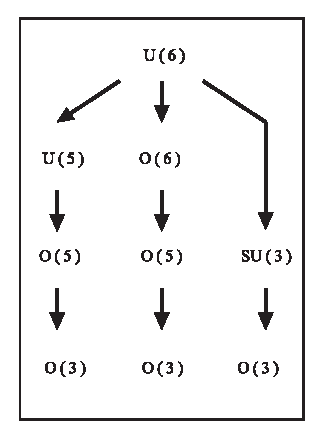
\includegraphics[scale=.65]{figure}
%
% If no graphics program available, insert a blank space i.e. use
%\picplace{5cm}{2cm} % Give the correct figure height and width in cm
%
%\caption{Please write your figure caption here}
\caption{If the width of the figure is less than 7.8 cm use the \texttt{sidecapion} command to flush the caption on the left side of the page. If the figure is positioned at the top of the page, align the sidecaption with the top of the figure -- to achieve this you simply need to use the optional argument \texttt{[t]} with the \texttt{sidecaption} command}
\label{fig:2}       % Give a unique label
\end{figure}

\runinhead{Run-in Heading Boldface Version} Use the \LaTeX\ automatism for all your cross-references and citations as has already been described in Sect.~\ref{sec:2}.

\subruninhead{Run-in Heading Italic Version} Use the \LaTeX\ automatism for all your cross-refer\-ences and citations as has already been described in Sect.~\ref{sec:2}\index{paragraph}.
% Use the \index{} command to code your index words
%
\begin{table}
\caption{Please write your table caption here}
\label{tab:1}       % Give a unique label
%
% Follow this input for your own table layout
%
\begin{tabular}{p{2cm}p{2.4cm}p{2cm}p{4.9cm}}
\hline\noalign{\smallskip}
Classes & Subclass & Length & Action Mechanism  \\
\noalign{\smallskip}\svhline\noalign{\smallskip}
Translation & mRNA$^a$  & 22 (19--25) & Translation repression, mRNA cleavage\\
Translation & mRNA cleavage & 21 & mRNA cleavage\\
Translation & mRNA  & 21--22 & mRNA cleavage\\
Translation & mRNA  & 24--26 & Histone and DNA Modification\\
\noalign{\smallskip}\hline\noalign{\smallskip}
\end{tabular}
$^a$ Table foot note (with superscript)
\end{table}

\begin{description}[Type 1]
\item[Type 1]{That addresses central themes pertainng to migration, health, and disease. Blablabla}
\item[Type 2]{That addresses central themes pertainng to migration, health, and disease. Blablabla}
\end{description}





\begin{acknowledgement}
If you want to include acknowledgments of assistance and the like at the end of an individual chapter please use the \verb|acknowledgement| environment -- it will automatically render Springer's preferred layout.
\end{acknowledgement}
%
%\section*{Appendix}
%\addcontentsline{toc}{section}{Appendix}
%


%%%%%%%%%%%%%%%%%%%%%%%% referenc.tex %%%%%%%%%%%%%%%%%%%%%%%%%%%%%%
% sample references
% %
% Use this file as a template for your own input.
%
%%%%%%%%%%%%%%%%%%%%%%%% Springer-Verlag %%%%%%%%%%%%%%%%%%%%%%%%%%
%
% BibTeX users please use
\bibliographystyle{abbrv}
\bibliography{bib,bib_gp}
%

%\begin{thebibliography}{99.}%
% and use \bibitem to create references.
%
% Use the following syntax and markup for your references if 
% the subject of your book is from the field 
% "Mathematics, Physics, Statistics, Computer Science"
%
% Contribution 
%\bibitem{science-contrib} Broy, M.: Software engineering --- from auxiliary to key technologies. In: Broy, M., Dener, E. (eds.) Software Pioneers, pp. 10-13. Springer, Heidelberg (2002)
%
% Online Document

%\end{thebibliography}

\end{document}
